\section{LITERATURE REVIEW}
\label{sec:literature_review}
\subsection{LiDAR}
The sensing system for automated vehicle navigation consists of a combination of active and passive sensors, i.e. camera, radar and lidar.
One such device, LIDAR, is an advanced active sensor system that illuminates and detects its surroundings by emitting lasers. Such devices accurately measure distances to various objects by emitting lasers and receiving them back from reflective surfaces. In a typical LiDAR system, one or more laser beams are scanned across its field of view. The generation and control of these laser beams relies on a sophisticated beam control system. The lasers are typically generated by modulated laser diodes that emit light at near-infrared (NIR) wavelengths. These laser beams are then reflected back by objects in the environment and the returned signals are captured by photodetectors on the scanner. Fast electronics in the lidar system filter these returned signals and measure the time difference between the emitted laser light and the received laser light. This time difference is the key to calculating the distance, as it is proportional to the distance. This time difference allows the system to accurately estimate the distance between the laser and the object. In addition, any variations in reflected intensity due to differences in surface materials or changes in environmental conditions between the transmitter and receiver can be compensated for by advanced signal processing techniques. The output of LiDAR is typically a point cloud of data that exhibits the structure of the scanned environment and includes information on the location of each point and the intensity of the reflected laser energy. This makes LiDAR extremely effective in environmental modelling and object recognition.
LiDAR ranging can work in two main ways: direct detection and coherent detection. Devices that use a pulsed laser directly measure distance by measuring the laser's time of flight (ToF); this type of device is called a direct detection laser rangefinder. The other type of device uses a Frequency Modulated Continuous Wave (FMCW) laser, which indirectly measures the distance and speed of an object through the Doppler effect, and this type of device is known as a coherent detection laser rangefinder.

\begin{figure}[H]
\centering
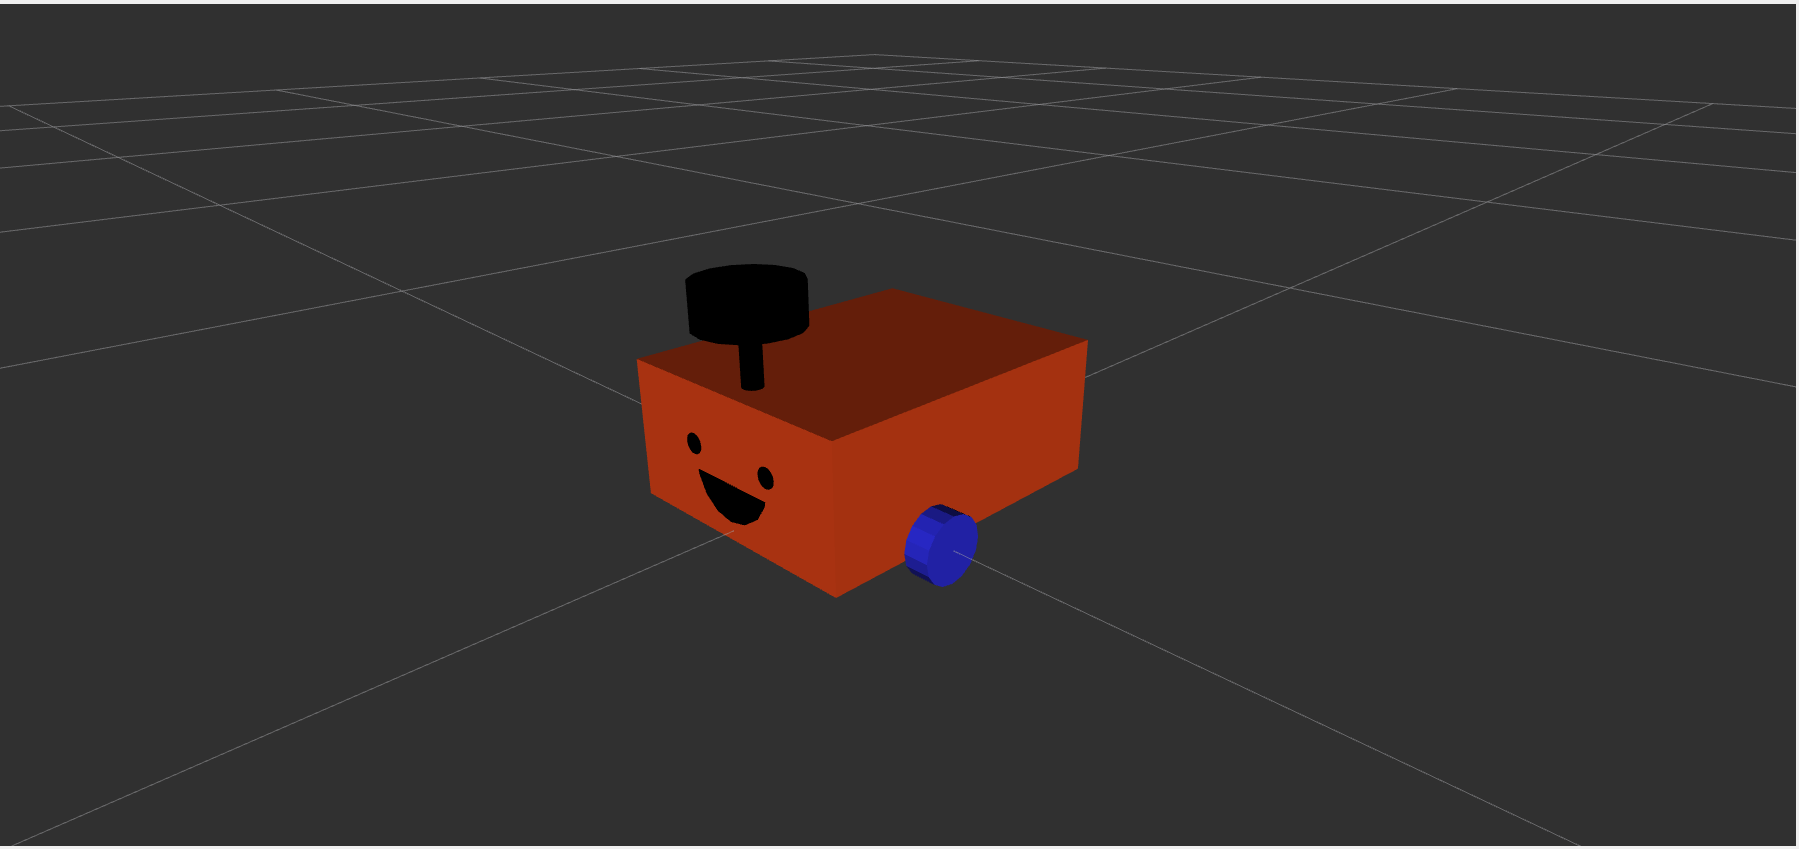
\includegraphics[width=0.8\linewidth]{figs/robot.png}
\caption{Example figure caption.}
\end{figure}

\subsection{Depth Camera}
Common depth cameras such as the Intel RealSense Camera utilise three lenses - a camera, an infrared (IR) camera and an IR projector - to assess depth by detecting infrared light reflected from the object/body in front of it. The resulting visual data is combined with software to create a depth estimate, i.e., a depth image is returned.

\begin{figure}[H]
\centering
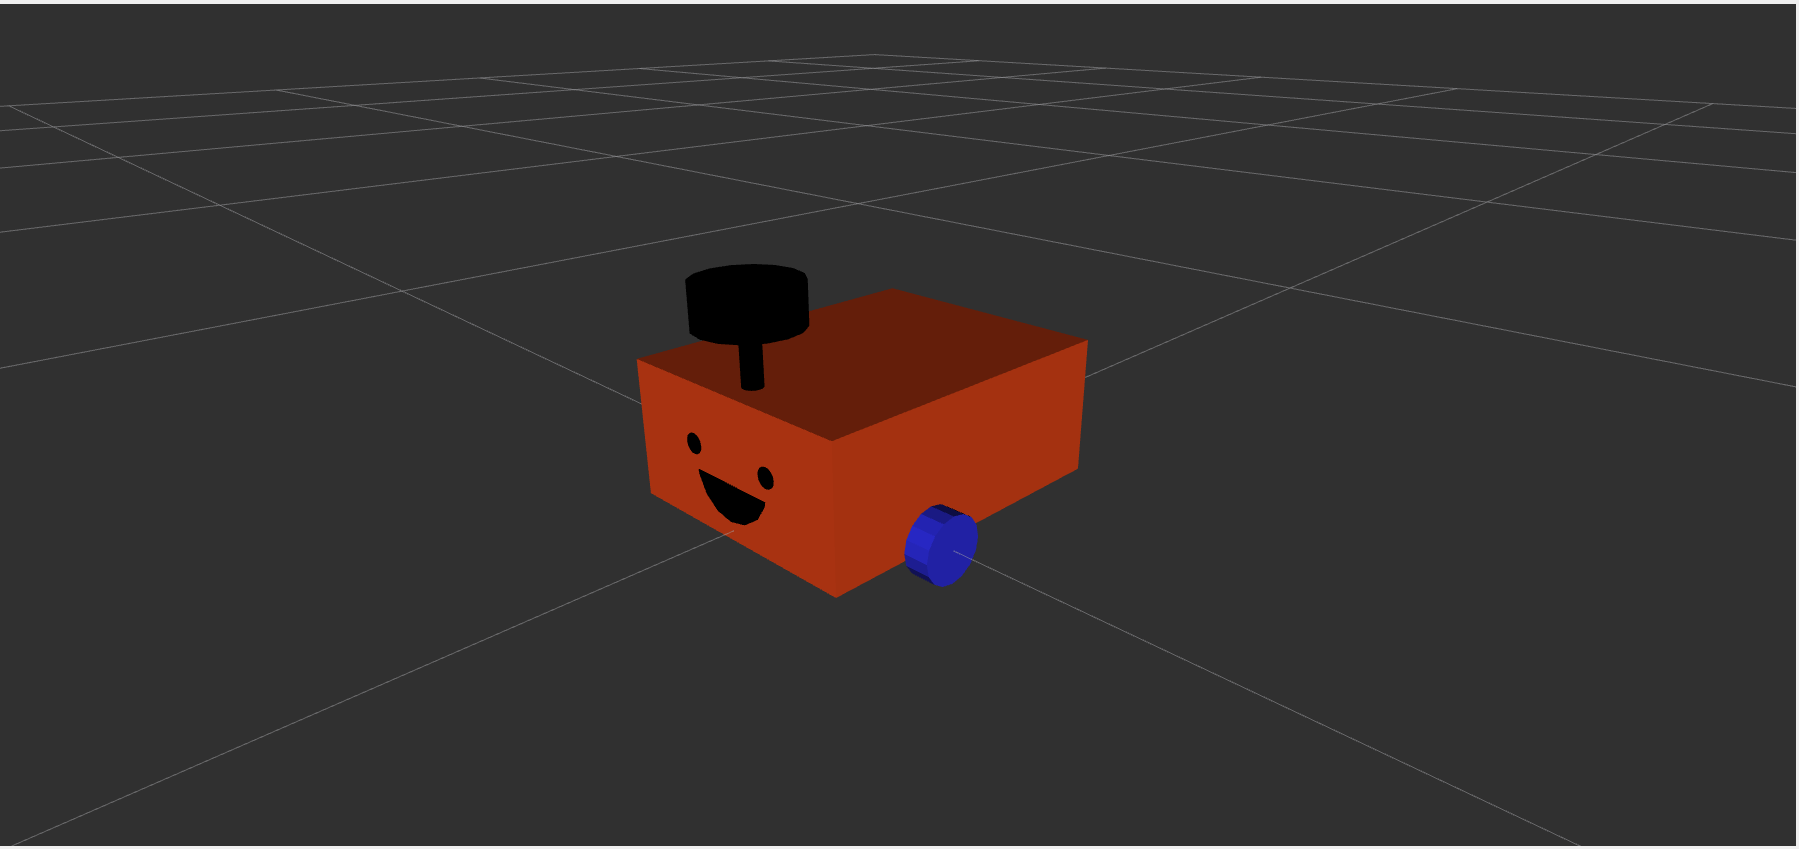
\includegraphics[width=0.8\linewidth]{figs/robot.png}
\caption{Example figure caption.}
\end{figure}
Different depth cameras use different techniques and mechanisms to achieve depth values. Stereo vision systems use two spaced apart cameras to capture images from slightly different angles, similar to human binocular vision. By comparing these two images, the system can calculate depth based on the difference between corresponding points in the images. Structured light technology involves projecting a pattern of light (usually infrared) onto a scene and capturing an image of it with a camera. Depth values are calculated by analysing the distortion of the light pattern caused by the surfaces in the scene, while the ToF camera emits pulses of light (usually infrared) and measures the time it takes for the light to travel to the object and return to the camera. This is very similar to the principle of LIDAR above
\subsection{SLAM}
The availability of accurate maps allows system designs to operate in complex environments based solely on their on-board sensors, without relying on external reference systems (e.g., GPS). Acquiring maps of indoor environments, often without GPS, has been a major research focus of the robotics community over the past decades. Learning maps under attitude uncertainty is often referred to as the simultaneous localisation and map building (SLAM) problem. It is a technique that enables robots to map unknown environments while simultaneously localising themselves based on the maps drawn, often in the absence of an external positioning system.
SLAM combines data from various sensors (e.g., cameras, LIDAR, inertial measurement units) to create a consistent map of the environment and determine the robot's position relative to that map. The process involves two main steps: localisation (estimating the robot's position in the environment) and mapping (constructing a model or map of the environment's layout).The SLAM algorithm relies heavily on odometry data, which involves measuring changes in position over time. In this project, detailed odometry information is provided by tracking the rotation of each wheel through a differential wheel. Differential steering provides the mobility and manoeuvrability required to navigate complex environments, and when used in conjunction with SLAM, enables precise navigation and obstacle avoidance in dynamic settings. Also, using only differential wheels as SLAM odometers can amplify the importance of obstacle avoidance for robots, which are very sensitive to collisions. This will be mentioned in the last part of Test.
\subsection{ROS2 Humble}
ROS 2 Humble Hawksbill is one of the versions of the Robotics Operating System (ROS 2), a successor to the original ROS (Robotics Operating System) designed to improve on the functionality of its predecessor, with a focus on new use cases in robotics, more robust communications, and support for real-time systems.
ROS2 Humble is used throughout this project for the following reasons: ROS 2 Humble is an LTS release, which means it will be supported and updated for a longer period of time. And when this project started, this version was the latest LTS version. Whilst it may be easier to find solutions within the ROS community when the project encounters problems using an earlier version, using a newer platform means that the project is more in line with the ongoing developments in the field of robotics, and thus easier to integrate with future technologies and standards emerging in the community. This is also a mission of this project.
\subsection{Nav2}
As the main objective of this project is to address the shortcomings of 2D LiDAR, it is important to use an auto-navigation method that is highly adapted to a wide range of sensors, is easy to use and has a robust performance.The Navigation2 framework is a state-of-the-art, open-source navigation stack that provides a comprehensive set of tools and libraries designed to enable autonomous navigation for a wide range of robotic platforms, especially in complex and dynamic environments. Nav2 is user-friendly and offers plug-and-play components that simplify the setup and configuration of advanced navigation systems in robots. It provides a wide range of navigation functions, including path planning, obstacle avoidance and map management. Its modular design makes it highly scalable.
\subsection{Gazebo}
Gazebo is a well-known open-source robotics simulator that offers a powerful physics engine, high-quality graphics, and a variety of sensors and objects that can be customised to mimic real-world scenarios. Moreover, Gazebo comes with a comprehensive library of sensor models and plug-ins to simulate cameras, LIDAR, and other common robot sensors. The entire simulator is fully integrated with the Robotics Operating System (ROS), making it an ideal tool for developing and testing ROS-based applications in a simulated environment. This project uses the Gazebo simulation world throughout to run, test and practice the algorithms. This reduces the risks and costs associated with physical prototyping. And algorithms and robot interactions can be tested in a variety of scenarios without causing expensive hardware damage. Through simulation, it is possible to quickly iterate on algorithm design, test changes, and see the results immediately. This rapid feedback loop significantly accelerates the development process.
\subsection{RViz2}
RViz is a powerful 3D visualisation tool for visualising sensor data, robot state and behaviour. The displays in RViz2 can be customised to meet different requirements, giving it the flexibility to adapt to all types of robotic applications. RViz2 is also fully integrated with ROS2 and can be used with Gazebo. RViz2 is used throughout this project to visualise data including robot models, trajectories, and sensor data streams (e.g. laser scans and cameras). It provides visual insights into what the robot is "seeing" and "thinking", which is essential for tuning algorithms and ensuring they perform as expected.
\subsection{Depthimage\_to\_Laserscan}
Depthimage\_to\_Laserscan is a ROS package that provides a basic solution for converting depth images from depth cameras to 2D laser scan data. Part of the code for converting depth image data to LaserScan data in the following section is adapted from this package. The details are explained in more detail below.
\subsection{Slam\_toolbox}
% TODO
\subsection{Proposed Solutions}
In the early stages of the project, two unique proposed solutions were also proposed and they are:
\subsubsection{YOLO-V8}
YOLO(You Only Look Once) is a deep learning model. It can detect objects, especially a wide variety of obstacles, with high accuracy and speed. Its superior efficiency enables robots to make fast, informed decisions about obstacle avoidance and path planning.
However, whilst YOLOv8 provides powerful target detection capabilities, it relies heavily on visual data from the camera. The aim of this project was to explore sensor fusion, in particular the integration of camera and LiDAR data, to take advantage of the complementary strengths of the two sensing modalities. YOLOv8 focuses only on camera input, which is not in line with the sensor fusion goals of this project.
\subsubsection{ORB-SLAM}
ORB-SLAM (Oriented FAST and Rotated BRIEF SLAM) is a versatile and accurate visual SLAM method that utilises a feature-based approach for simultaneous localisation and mapping. It can construct detailed environmental maps and accurately locate vehicles in environments not recognised by GPS.
While ORB-SLAM is somewhat able to address the problem of map-building crashes due to collisions for robots using only differential wheel odometers, it is not primarily designed for dynamic obstacle detection and avoidance. Its focus on creating a static map of the environment, rather than consistently recognising and bypassing transient obstacles, is also at odds with the goals of the project.
